\subsection{Model Selection} \label{meth-synth-model-subsect}
To perform \emph{model selection} the Bayesian Information Criterion (BIC) \citep{Schwarz1978} can be used. BIC is a popular measure for comparing maximum likelihood models and is defined as:
\begin{equation}
	BIC = -2 \times \log (\text{likelihood}) + k \times \log (N)
\end{equation}
where $N$ is the number of objects and $k$ is the total number of parameters to be estimated. The model with the highest BIC score is preferred.

\emph{Fig. \ref{BIC:first}} shows how BIC score changes as we increase the number of clusters K, for a $3^{rd}$ degree polynomial. For K=3 clusters the model reaches the highest BIC score, which is the optimal selection for the model. \emph{Fig. \ref{BIC:second}} shows the change of BIC score as we increase the degree of the polynomial for K=3 clusters. The optimal model choice is using a $4^{th}$ degree polynomial.
\begin{figure}[ht!]
     \begin{center}
        \subfigure[]{
            \label{BIC:first}
            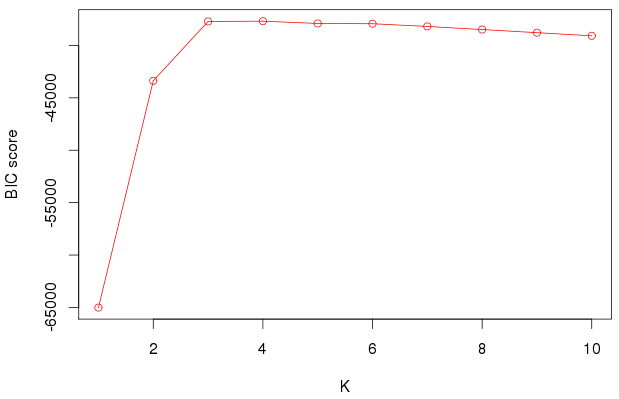
\includegraphics[width=0.45\textwidth]{images/BIC-K}
        }
        \subfigure[]{
           \label{BIC:second}
           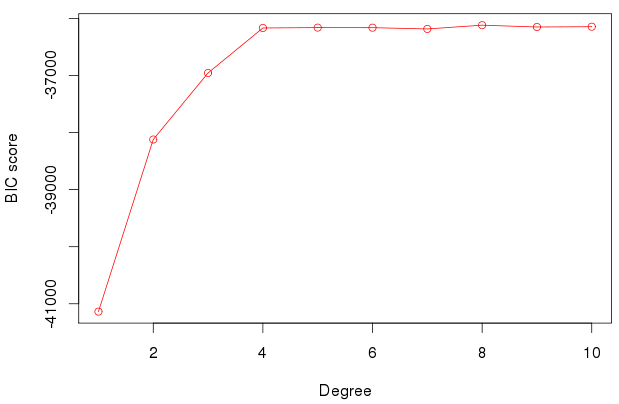
\includegraphics[width=0.45\textwidth]{images/BIC-Deg}
        }
    \end{center}
    \caption{\emph{(a) BIC score as the number of clusters K increases, for a $3^{rd}$ degree polynomial. (b) BIC score as the degree of polynomial increases for K=3 clusters.}}
   \label{BIC-pic}
\end{figure}